\documentclass[a4paper, titlepage, 12pt, norsk]{article}

\usepackage[utf8]{inputenc} % For å kunna skriva æøå i tekstar
\usepackage[T1]{fontenc}
\usepackage[margin=2cm]{geometry} % Fiksa margin
\usepackage[ddmmyyyy]{datetime} % Fiksar datorormatet på tiitelen
\usepackage{amssymb}
\usepackage{amsmath} % For visse mattesymbol, typ \mathbb
\usepackage{graphicx} % Bilete
%\usepackage{minted} % For kodesnuttar og resultat
\usepackage{enumitem} % Kan endra på korleis listar ser ut

\usepackage[hidelinks,colorlinks=true]{hyperref} % For autoref
\hypersetup{allcolors=[rgb]{0,0.31,0.62}}

\usepackage{amsthm}
\usepackage{thmtools} 

\usepackage{tikz}
\usetikzlibrary{matrix}
\newcommand{\diagram}[3]{\matrix (#1) [matrix of math nodes,row
  sep={#2},column sep={#3},text height=1.5ex,text
  depth=0.25ex]}

\RequirePackage{fontspec}
\setmainfont{Atkinson Hyperlegible}

% Ny type lista med ganske perfekt spacing
\newlist{plist}{enumerate}{5}
\setlist[plist]{align=left, itemindent = 0cm, labelsep = 0cm, labelindent = 0cm}
\setlist[plist,1]{label=\arabic*, font=\bf\Large}
\setlist[plist,2]{label*=.\arabic*, labelwidth=1.25cm, leftmargin=1.25cm}
\setlist[plist,3]{label*=.\arabic*, labelwidth=1.5cm, leftmargin=1.5cm}

\theoremstyle{plain}
\newtheorem{theorem}{Teorem}[section]
\newtheorem{proposition}[theorem]{Proposjon}
\newtheorem{corollary}[theorem]{Korollar}
\newtheorem{lemma}[theorem]{Lemma}

\theoremstyle{definition}
\newtheorem{definition}[theorem]{Definisjon}
\newtheorem{example}[theorem]{Eksempel}
\newtheorem{remark}[theorem]{Merknad}

\usepackage[norsk]{babel}
%\renewcommand*{\proofname}{Bevis}

\newcommand{\R}{\mathbb{R}}
\newcommand{\Q}{\mathbb{Q}}
\newcommand{\Z}{\mathbb{Z}}
\newcommand{\N}{\mathbb{N}}

\title{Nerveteorement og Anvendingar}
\author{Håvard Skjetne Lilleheie}

\begin{document}

\maketitle

\section{Grunnleggande definisjonar og resultat}

\begin{definition}
	For $V$ ei ikkje-tom og endeleg mengda, så definerar me $K$ til å vera eit \emph{endeleg asbtrakt simplisielt kompleks over $V$} om:
	\begin{enumerate}
		\item{$\forall v \in V: \{v\} \in K$}
		\item{$\forall \sigma \in K, \forall \tau \subseteq \sigma: \tau \in K$}
	\end{enumerate}
	Då kallar me og $V$ for \emph{hjørnemengda} til $K$.
\end{definition}
\noindent Nokre eksempel av endelege abstrakte simplisielle kompleks over $\{p_1, p_2, p_3\}$:
\begin{itemize}
	\item{$A_1=\{\{p_1, p_2\}, \{p_1\}, \{p_2\}\}$}
	\item{$A_2=\{\{p_1\}, \{p_2\}, \{p_3\}, \{p_1, p_3\}, \{p_2, p_3\}\}$}
	\item{$A_3=\{\{p_1\}, \{p_2\}, \{p_3\}\}$}
\end{itemize}
Og her er nokre ikkje-eksempel av endelege abstrakte simplisielle kompleks over $\{p_1, p_2, p_3\}$:
\begin{itemize}
	\item{$A_1'=\{\{p_1, p_2\}, \{p_1\}\}=A_1 \setminus \{\{p_2\}\}$}
	\item{$A_2'=\{\{p_1\}, \{p_2\}, \{p_3\}, \{p_1, p_3\}, \{p_2, p_3\}, \{p_1, p_2, p_3\}\}=A_2 \cup \{\{p_1, p_2, p_3\}\}$}
	\item{$A_3'=\{\{p_1\}, \{p_2\}, \{p_2, p_3\}\}=\left(A_3 \setminus \{\{p_3\}\}\right) \cup \{\{p_2, p_3\}\}$}
\end{itemize}
Inspirasjonen bak denne definisjonen kan verka tilfeldig og heilt umotivert, men som me kjem til å sjå seinare; så er dette ein svært praktisk simplifisering av informasjon som bevarer mykje av eigenskapane til den originale datamengda ein vil sjå på. 
\\Fyrst, lat oss sjå korleis dette kan tenkast på som meir geometrisk:
\begin{definition}
	Ein endeleg mengda punkt $\{p_1, p_2, p_3, \dots, p_n\}$ i $\R^m$ for $m\geq1$ er \emph{geometrisk uavhengige} om for $\{a_i\}_{i=0}^n$ med $a_i\in\R$, så:
	\begin{equation*}
		\left(\sum_{i=1}^n a_i=0 \land  \sum_{i=1}^n a_ip_i=0\right)\Rightarrow a_i=0 \; \forall i
	\end{equation*}
\end{definition}
\begin{theorem}\label{thm:geometrisklineærtuavhengig}
	Ei endeleg mengda $\{p_1, p_2, p_3, \dots, p_n \}$ av punkt i $\R^m$ er gemetrisk uavhengige $\Leftrightarrow$ vektorane $\{(p_2-p_1), (p_3-p_1), (p_4-p_1),\dots,(p_n-p_1)\}$ er lineært uavhengige i $\R^m$
\end{theorem}
\begin{proof}
	(\Rightarrow)
	\\For $a_i\in\R$, annta $\sum_{i=2}^na_i(p_i-p_1)=0$. Om me då definerar: $a_1 := -\sum_{i=2}^na_i$, så ser me at 
	\begin{equation*}
		\sum_{i=1}^na_i=\sum_{i=2}^na_i-\sum_{i=2}^na_i=0
	\end{equation*}
	og at 
	\begin{equation*}
		\sum_{i=1}^na_ip_i=\sum_{i=2}^na_i(p_i-p_1)=0
	\end{equation*}
	Og sidan $\{p_i\}_{i=1}^n$ er geometrisk uavhengig frå antaginga, så $\Rightarrow$ $a_i=0 \, \forall i$. Som er definisjonen på lineært uavhengig.
	\\(\Leftarrow)
	\\for $a_i\in\R$, annta $\sum_{i=1}^n a_i=0$ og $\sum_{i=1}^n a_ip_i=0$. Då ser me at 
	\begin{equation*}
		a_1=-\sum_{i=2}^n a_i
	\end{equation*} 
	Det gir oss: 
	\begin{equation*}
		0=\sum_{i=1}^n a_ip_i=\sum_{i=2}^n a_ip_i-\sum_{i=2}a_ip_1=\sum_{i=2}a_i(p_i-p_1)
	\end{equation*}
	Men sidan $\{(p_i-p_1)\}_{i=2}^n$ er lineært uavhengig, så: $\Rightarrow a_i = 0$ for $i\in[2,n]$. Men sidan $a_1 = -\sum_{i=2}^n a_i=0$, så får me $a_i=0 \forall i$. Som er definisjonen på geometrisk uavhengig.
\end{proof}
\begin{remark}
	Ein direkte konsekvens frå dette resultatet og grunnleggande lineær algebra er at ein geometrisk uavhengig mengda i $\R^m$ kan maksimalt innehalda $m+1$ forskjellige punkt. Dette er fordi det kan ikkje vera meir enn $m$ lineært uavhengige vektorar i eit $m$-dimensjonalt vektorrom.
\end{remark}
\begin{definition}
	Ein \emph{konveks kombinasjon} av ei geometrisk uavhengig mengda $P=\{p_1, p_2, p_3, \dots, p_n\}$ av punkt i $\R^m$ er eit punkt $x\in\R^m$ gitt ein tupel av koeffisientar $A=\{a_1, a_2, a_3, \dots, a_n\}$ i $\R$, med $a_i\geq0\forall i$ og $\sum_{i=1}^n a_i = 1;$
	\begin{equation*}
		x=\sum_{i=1}^n a_ip_i
	\end{equation*}
%	Om $P$ er ein tupel (ein ordna mengda) så blir koeffiseintane også ein tupel, og $A$ blir då kalla dei \emph{barysentriske koordinatane} til $x$.
\end{definition}
%\begin{theorem}
%	Dei barysentriske koordinatane til ein konveks kombinasjon er eintydig.
%\end{theorem}
%\begin{proof}
%	La $x$ vera ein konveks kombinasjon av $(p_1, p_2, p_3, \dots, p_n)$ i $\R^m$. Annta at $x$ har to barysentriske koordinatar: $(a_1, a_2, a_3, \dots, a_n)$ og $(b_1, b_2, b_3, \dots, b_n)$. Det betyr at:
%	\begin{equation*}
%		0 = x - x = \sum_{i=1}^n a_ip_i - \sum_{i=1}^n b_ip_i=\sum_{i=1}^n (a_i-b_i)p_i
%	\end{equation*}
%	og me får:
%	\begin{equation*}
%		\sum_{i=1}^n(a_i-b_i)=\sum_{i=1}^na_i - \sum_{i=1}^nb_i = 1 - 1 = 0
%	\end{equation*}
%	Men sidan $(p_1, p_2, p_3, \dots, p_n)$ er geometrisk uavhengig, så 
%	\begin{equation*}
%		\Rightarrow (a_i-b_i)=0\forall i \Leftrightarrow a_i = b_i \forall i
%	\end{equation*}
%	og dei barysentriske koordinatane er derfor like.
%\end{proof}
\begin{definition}
	Det \emph{geometrisk simplekset} utspent av ei geometrisk uavhengig mengda av punkt $P=\{p_1, p_2, p_3, \dots, p_n\}$ i $\R^m$, er alle konvekse kombinasjonar av $P$.
	\\Vidare, så kallar me dette geometriske simplekset for eit \emph{$(n-1)$-simpleks}, når $P$ består av $n$ punkt.
\end{definition}
\begin{remark}
	Ut ifrå den førre definisjonen så ser me at eit $0$-simpleks kun er eit enkelt punkt, eit $1$-simpleks er alle konvekse kombinasjonar mellom to punkt, som viser seg å vera ei linja mellom dei to punkta. Og eit $2$-simpleks dannar ein trekant. Ein $3$-simpleks blir også kalla eit tetraheder. Denne simpleks definisjonenen gir ein fin matematisk forklaring av "trekant"-strukturar i $\R^m$.
\end{remark}
\begin{remark}
	Noko som er svært interessant med denne definisjonen er at om ein har ei geometrisk uavhengig mengda $P$, og ser på $P^i := P \setminus \{p_i\}$, så vil dette også vera ei geometrisk uavhengig mengda. I tilleg så vil det geometriske simplekset utspent av $p^i$ vere ei delmengda av det geometriske simplekset utspent av $P$. Med andre ord; alle delmengdar av $P$ dannar også andre geometriske simpleks, inneholdt i det originale geometriske simplekset! Men ikkje nok med det, fordi når ein ser på det geometriske simplekset utspent av $P^i$ for ein eller annan vilkårleg $i$, så ser me at det er som eine "fjeset" av det geometriske simplekset utspunne av $P$. Dette inspirerar ein ny definisjon:
\end{remark}
\begin{definition}
	Eit \emph{fjes} til eit geometrisk simpleks utspunne av $P=\{p_1, p_2, p_3, \dots, p_n\}$ er eit geometriske simpleks utspunne av $P^i := P\setminus \{p_i\}$ for ein eller annan $i$.
\end{definition}
\begin{definition} % Ikkje utspunne av nokre punkt?
	Eit \emph{geometrisk simplisielt kompleks} er ei mengda av geometriske simpleksar (utspent av punkt i $\R^m$), $K$, sånn at:
	\begin{enumerate}
		\item{For $\sigma \in K$ så er alle fjesa til $\sigma$ også i $K$.}
		\item{For $\sigma, \tau \in K$ med $\sigma \cap \tau \neq \emptyset$, då er $\sigma \cap \tau$ eit fjes av både $\sigma$ og $\tau$.}
	\end{enumerate}
\end{definition}
\begin{definition}
	For $V$ ein endeleg mengda og $m\geq1$, så er $f:V\rightarrow \R^m$ ein \emph{affin imbedding} om $f$ er injektiv, og om biletet, $f(A)$ er ei geometrisk uavhengig mengda av punkt.
\end{definition}
\begin{definition}
	For eit endeleg abstrakt simplisielt kompleks $K$, over ei ikkje-tom hjørnemengda $V$, gitt ein vilkårleg affin imbedding $f:V\to\R^m$ for ein eller annan $m\geq1$. Så er den \emph{geometriske realiseringa med hensyn til $f$} unionen av alle dei geometriske simpleksane utspunne av punkta i $f(\sigma)$, for $\sigma\in K$. Dette er ofte betegna $|K|_f$
\end{definition}
\begin{theorem}
	Geometrisk realisering er eintydig opp til homeomorfi. Med andre ord: For to ulike geometriske realiseringar av eit endeleg abstrakt simplisielt kompleks $K$, med hensyn til $f$ og $g$ (to ulike affine imbeddingar), så er $|K|_f$ og $|K|_g$ homeomorfe.
\end{theorem}
\begin{proof}%Rotete? Trenge unike barysentriske koordinatar? Må visa \hat{\tau} er bijeksjonar
	La $K$ vera eit abstrakt simplisielt kompleks, og la $f:K\to\R^m$ og $g:K\to\R^l$ vera to affine imbeddingar. La $V={v_1, v_2, \dots, v_n}$ vera hjørnemengda til $K$ Definér vidare $x_i=(f(k_{i-1})-f(k_1))$ og $y_i=(g(k_{i-1})-g(k_1))$. La $\tau_f:\R^m\to\R^m$ vera ein translasjon som tek $x\mapsto x-f(k_1)$. Og la $\tau_g:\R^l\to\R^l$ vera ein translasjon som tek $x\mapsto x-g(k_1)$. Til slutt, la $L_1:\R^m\to\R^l$ vera den lineære funksjonen som sender $x_i\mapsto y_i$.
Og for praktiske grunnar: Definér $\hat{f}:=\tau_f\circ f$ og $\hat{g}:=\tau_g \circ g$
Me får då at $L_1(\hat{f}(k_i))=\hat{g}(k_i)$, fordi:
For $i=1$:
\begin{equation*}
	L_1(\hat{f}(k_1)=L_1(f(k_1)-f(k_1))=L(0)=0=g(k_1)-g(k_1)=\hat{g}(k_1)
\end{equation*}
For $i\neq 1$:
\begin{equation*}
	L_1(\hat{f}(k_i))=L_1(f(k_i)-f(k_1))=L_1(x_{i-1})=y_{i-1}=g(k_i)-g(k_1)=\hat{g}(k_i)
\end{equation*}
Om ein då let $\hat{L}=L|_{|K|_{\hat{f}}}$, og $L_2:\R^l\to\R^m$ vera den lineære funskjonen som sender $y_i\mapsto x_i$ og let $\tilde{L}=L_2|_{|K|_{\hat{g}}}$, så er definisjonane symmetriske og det symmetriske resultatet gjelder derfor for $L_2$ også. 
For eit vilkårleg element $x\in|K|_{\hat{f}}$ så er $x$ eit element av ein simpleks i det geometriske simplisielle komplekset. Det vil seie, me kan utrykka $x$ som ein konveks sum av ein geometrisk uavhengig mengda, som korresponderar til den simpleksen $x$ er eit element i.
\\Me velger derfor ein $\sigma\in K$ sånn at $\hat{f}(\sigma)=\{\hat{f}(k_1), \hat{f}(k_2), \dots, \hat{f}(k_r)\}$. Dette er ein geometrisk uavhengig mengda fordi $\tau_f$ er injektiv og sender $x_i\mapsto x_i$ som er lineært uavhengig og biletet er derfor geometrisk uavhengig om $\{x_i\}$ er lineært uavhengig, som det er frå \autoref{thm:geometrisklineærtuavhengig}.
\\La denne mengda utspenna punkta til ein simpleks som $x$ er eit element av. Då kan me utrykka $x$ som ein konveks kombinasjon av elementa i $\hat{f}(\sigma)$: $x=\sum_{i=1}^ka_i\hat{f}(k_i)$ med $\sum_{i=1}^ka_i=1$ og $a_i\geq0\; \forall i$. 
\\Her er valet av kva geometrisk simpleks me velger ikkje vikitg, ettersom $\hat{L}$ er veldefinert.
\begin{align*}
	\tilde{L}\circ \hat{L}(x) &= \tilde{L}\circ \hat{L}\left(\sum_{i=1}^ra_i\hat{f}(k_i)\right) \\
	&= \tilde{L}\left(\sum_{i=1}^r\hat{L}(a_i\hat{f}(k_i))\right) \\
	&= \tilde{L}\left(\sum_{i=1}^ra_i\hat{L}(\hat{f}(k_i))\right) \\
	&= \tilde{L}\left(\sum_{i=1}^ra_i\hat{g}(k_i))\right) \\
	\intertext{Sidan $\sum_{i=1}^ra_i\hat{g}(k_i)\in|K|_{\hat{g}}$, så får me:} \\
	&= \sum_{i=1}^r\tilde{L}(a_i\hat{g}(k_i)) \\
	&= \sum_{i=1}^ra_i\tilde{L}(\hat{g}(k_i)) \\
	&= \sum_{i=1}^ra_i\hat{f}(k_i) \\
	&= x
\end{align*}
Og likt for $\hat{L}\circ\tilde{L}(y)$.
Så det betyr at $\hat{L}$ er bijektiv med invers $\tilde{L}$.
Om ein let $\hat{\tau}_f:=\tau_f|_{|K|_f}$ og $\hat{\tau}_g:=\tau_g|_{|K|_g}$, så får ein følgande kommutative diagram:
\begin{center}
	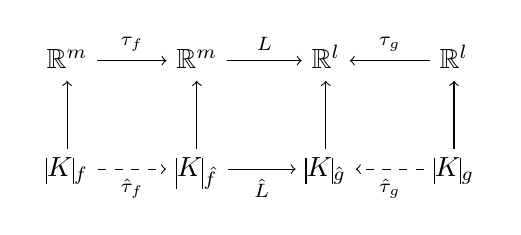
\begin{tikzpicture}
		\diagram{d}{2.5em}{2.5em}{
			\R^m & \R^m & \R^l & \R^l \\
			\vline K\vline_f & \vline K\vline_{\hat{f}} & \vline K\vline_{\hat{g}} & \vline K\vline_g \\
			};
	\path[->,font = \scriptsize, midway]
	(d-1-1) edge node[above]{$\tau_f$} (d-1-2)
	(d-1-2) edge node[above]{$L$} (d-1-3)
	(d-1-4) edge node[above]{$\tau_g$} (d-1-3)
	(d-2-1) edge [dashed,->] node[below]{$\hat{\tau}_f$}(d-2-2)
	(d-2-2) edge node[below]{$\hat{L}$} (d-2-3)
	(d-2-4) edge [dashed,->] node[below]{$\hat{\tau}_g$} (d-2-3)
	(d-2-1) edge (d-1-1)
	(d-2-2) edge (d-1-2)
	(d-2-3) edge (d-1-3)
	(d-2-4) edge (d-1-4);
	\end{tikzpicture}
\end{center}
Der alle vertikale avbildningane er den naturlege inklusjonen.
Merk her at ettersom den naturlege inklusjonen er kontinuerlig, så er alle avbildningane på nederste rad også kontinuerlige frå at diagrammet kommuterar og definisjonen av underromstopologien. Meir spesifikt, så får ein at sidan $\tau_f$ og $\tau_g$ er homeomorfiar, at dei induserte avbildningane gitt av dei prikka linjene også er homeomorfiar.
Og sidan $\hat{L}$ er både kontinuerlig og bijektiv, med invers $\tilde{L}$ som frå eit symmetrisk argument også er kontinuerlig, at $\hat{L}$ er ein homeomorfi.
Så me får ein avbildning: $(\tau_g)^{-1}\circ\hat{L}\circ\tau_f:|K|_f\to|K|_g$ som er ein samansetting av tre homeomorfiar, og er derfor ein homeomorfi sjølve.
\end{proof}
\begin{remark}
	Grunna det førre resultatet så er det vanleg å snakka om \emph{den} geometriske realiseringa til eit abstrakt simplisielt kompleks $K$, ettersom alle forskjellige geometriske realiseringar er homeomorfe. Derfor plar ein ofte å sløyfa subskrifta i notasjona og kun bruka $|K|$ for \emph{den} geometriske realiseringa til $K$.
\end{remark}



\end{document}
